\graphicspath{{./images/}}

\chapter{Kontextabgrenzung}

\section{Fachlicher Kontext}

\begin{figure}[H]
	\centering
	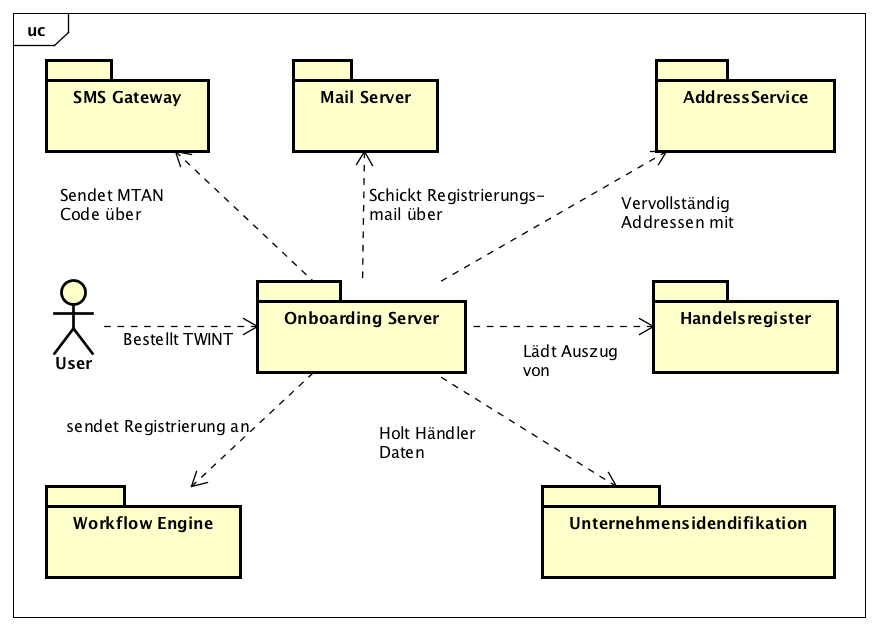
\includegraphics[scale=0.6]{Contextdiagramm.png}
	\caption{Fachliche Kontext}
\end{figure}

\section{Technischer Kontext}

Der Onboarding Server verwendet Spring Boot, das Frontend AngularJS und die Workflow Engine Camunda zusammen mit Wildfly. Die Anwendung wird mittels der Container Technologie Docker auf der OpenShift Container Plattform ausgerollt. 

\section{Externe Schnittstellen}

\subsection{UID Schnittstelle}

\begin{table}[H]
	\centering
	\caption{UID-Schnittstelle}
	\begin{tabular}{ | p{4cm} | p{11cm} | }
		\toprule
		{\textbf{Name}} & {\textbf{Beschreibung}} \\
		\midrule
		Identifikation & \textit{\gls{URL}}\\ \hline
		Bereitgestellte Resource & Erlaubt das Abfragen von Unternehmensdaten anhand der Unternehmensidentifikationsnummer. \\ \hline
		Fehlerszenarien & Ist die Schnittstelle nicht verfügbar, muss der Händler die Daten selber eingeben welche falsch sein könnte.\\ \hline
		Qualitätseigenschaften & Maximal 20 Anfragen pro Minuten sonst wird der sender geblockt.  Garantierte Verfügbarkeit von 362 Tagen \url{https://www.isb.admin.ch/isb/de/home/e-services-bund/services/uid-webservice.html}\\ \hline
		Entwurfsentscheidungen & Falls die Schnittstelle nicht verfügbar ist, werden die Buttons im User Interface ausgeblendet.\\
		\bottomrule
	\end{tabular}
\end{table}

Weitere Informationen zur Schnittstelle finden sich in Kapitel \ref{documents} D-1

\subsection{ZEFIX Schnittstelle}

\begin{table}[H]
	\centering
	\caption{ZEFIX-Schnittstelle}
	\begin{tabular}{  | p{4cm} | p{11cm} | }
		\toprule
		{\textbf{Name}} & {\textbf{Beschreibung}} \\
		\midrule
		Identifikation & \textit{\gls{URL}}\\ \hline
		Bereitgestellte Resource & Abfrage des Handelsregisterauszugs \\ \hline
		Fehlerszenarien & Ist die Schnittstelle nicht verfügbar, muss der Händler den Auszugs selber hochladen.\\ \hline
		Entwurfsentscheidungen & Falls die Schnittstelle nicht verfügbar ist, werden die Buttons im User Interface ausgeblendet.\\
		\bottomrule
	\end{tabular}
\end{table}

Weitere Informationen zur Schnittstelle finden sich in Kapitel \ref{documents} D-3

\subsection{Adressen Schnittstelle}

\begin{table}[H]
	\centering
	\caption{Address-Schnittstelle}
	\begin{tabular}{  | p{4cm} | p{11cm} |}
		\toprule
		{\textbf{Name}} & {\textbf{Beschreibung}} \\
		\midrule
		Identifikation & \textit{\gls{URL}} \\ \hline
		Bereitgestellte Resource & Plz/Ort und Strasse für die Autovervollständigung im XML Format \\ \hline
		Fehlerszenarien & Ist die Schnittstelle nicht verfügbar, muss der Händler die Adressdaten selber eingeben.\\ \hline
		Entwurfsentscheidungen & Falls die Schnittstelle nicht verfügbar ist, werden die Buttons im User Interface ausgeblendet.\\
		\bottomrule
	\end{tabular}
\end{table}

Weitere Informationen zur Schnittstelle finden sich in Kapitel \ref{documents} D-2

\subsection{Mail Schnittstelle}

\begin{table}[H]
	\centering
	\caption{Mail-Schnittstelle}
	\begin{tabular}{ | p{4cm} | p{11cm} |}
		\toprule
		{\textbf{Name}} & {\textbf{Beschreibung}} \\
		\midrule
		Identifikation & \textit{\gls{URL}} \\ \hline
		Bereitgestellte Resource & Versenden von E-Mails\\ \hline
		Fehlerszenarien & Mail Server ist nicht erreichbar. Mail wurde an Mail Server verschickt welcher das Mail aber nicht weiter verschickt hat.\\ \hline
		Entwurfsentscheidungen & Wenn die Verbindung zum Mailserver nicht funktioniert, wird eine Fehlermeldung angezeigt. Sollte der Mail Server die Mail nicht weiter schicken, soll die Mail an eine separate Mailbox gesendet werden damit der Fehler behandelt werden kann.\\
		\bottomrule
	\end{tabular}
\end{table}

\subsection{ATMS Schnittstelle}

\begin{table}[H]
	\centering
	\caption{ATMS-Schnittstelle}
	\begin{tabular}{ | p{4cm} | p{11cm} | }
		\toprule
		{\textbf{Name}} & {\textbf{Beschreibung}} \\
		\midrule
		Identifikation & \textit{\gls{URL}} \\ \hline
		Bereitgestellte Resource & Versenden von E-Mails\\ \hline
		Fehlerszenarien & SMS Server nicht erreichbar oder Nummer ist falsch.\\ \hline
		Entwurfsentscheidungen & Fehlermeldung wird dem Benutzer angezeigt, dass der Server nicht erreichbar ist respektive das SMS nicht gesendet werden konnte.\\
		\bottomrule
	\end{tabular}
\end{table}

Weitere Informationen zur Schnittstelle finden sich in Kapitel \ref{documents} D-4
